\chapter{线性代数基础}

\intro{线性代数是深度学习的数学基石。神经网络的前向传播本质上是矩阵乘法与非线性激活的交替，反向传播则依赖于梯度在计算图中的传播。本章系统介绍深度学习所需的线性代数知识，包括标量、向量、矩阵、张量的基本概念，矩阵运算，范数，特征分解与奇异值分解等核心内容。}

\section{标量、向量与矩阵}

\subsection{标量}

标量（Scalar）是一个单独的数值，通常用小写斜体字母表示，如 $a$、$n$、$x$。在深度学习中，标量常用于表示损失函数值、学习率、准确率等单一数值。

\subsection{向量}

向量（Vector）是一组有序的数值，可视为一维数组。本书约定向量用粗体小写字母表示，如 $\mathbf{x}$。一个 $n$ 维向量可以表示为：

\[
\mathbf{x} = \begin{bmatrix} x_1 \\ x_2 \\ \vdots \\ x_n \end{bmatrix} \in \R^n
\]

向量的第 $i$ 个元素记为 $x_i$。在深度学习中，向量常用于表示单个样本的特征、权重参数等。例如，一张 $28\times 28$ 的灰度图像可以被展平为一个 $784$ 维向量。

\begin{mycode}{Python中的向量操作}
\begin{lstlisting}[language=Python]
import numpy as np

# 创建向量
x = np.array([1.0, 2.0, 3.0, 4.0])
print(f"向量: {x}")
print(f"维度: {x.shape}")
print(f"第2个元素: {x[1]}")

# 向量基本运算
y = np.array([5.0, 6.0, 7.0, 8.0])
print(f"加法: {x + y}")
print(f"标量乘法: {2.0 * x}")
print(f"点积: {np.dot(x, y)}")
print(f"逐元素乘积: {x * y}")
\end{lstlisting}
\end{mycode}

\subsection{矩阵}

矩阵（Matrix）是一个二维数组，用粗体大写字母表示，如 $\mathbf{A}$。一个 $m$ 行 $n$ 列的矩阵记为：

\[
\mathbf{A} = \begin{bmatrix}
a_{11} & a_{12} & \cdots & a_{1n} \\
a_{21} & a_{22} & \cdots & a_{2n} \\
\vdots & \vdots & \ddots & \vdots \\
a_{m1} & a_{m2} & \cdots & a_{mn}
\end{bmatrix} \in \R^{m\times n}
\]

矩阵的重要属性：
\begin{itemize}
    \item \textbf{转置}（Transpose）：将矩阵的行和列互换，记为 $\mathbf{A}^{\top}$。若 $\mathbf{A}\in\R^{m\times n}$，则 $\mathbf{A}^{\top}\in\R^{n\times m}$，且 $(\mathbf{A}^{\top})_{ij}=A_{ji}$。
    \item \textbf{对称矩阵}：若 $\mathbf{A}=\mathbf{A}^{\top}$，则 $\mathbf{A}$ 为对称矩阵。
    \item \textbf{对角矩阵}：只有主对角线上的元素可能非零，其余元素均为零。
    \item \textbf{单位矩阵}：主对角线全为 $1$ 的对角矩阵，记为 $\mathbf{I}_n$。
    \item \textbf{逆矩阵}：若存在矩阵 $\mathbf{A}^{-1}$ 使得 $\mathbf{A}\mathbf{A}^{-1}=\mathbf{I}$，则称 $\mathbf{A}$ 可逆。
\end{itemize}

\begin{mycode}{Python中的矩阵操作}
\begin{lstlisting}[language=Python]
import numpy as np

# 创建矩阵
A = np.array([[1, 2, 3],
              [4, 5, 6],
              [7, 8, 9]])
print(f"矩阵 A:\n{A}")
print(f"A 的形状: {A.shape}")
print(f"A 的转置:\n{A.T}")

# 单位矩阵
I = np.eye(3)
print(f"单位矩阵:\n{I}")

# 矩阵乘法
B = np.array([[2, 0, 1],
              [0, 3, 2],
              [1, 1, 0]])
C = A @ B  # 或 np.dot(A, B)
print(f"A @ B:\n{C}")

# 逐元素乘法（Hadamard积）
D = A * B
print(f"A * B (Hadamard积):\n{D}")
\end{lstlisting}
\end{mycode}

\subsection{张量}

张量（Tensor）是标量、向量和矩阵向更高维度的推广。标量是零阶张量，向量是一阶张量，矩阵是二阶张量。在深度学习中，常见的张量包括：

\begin{itemize}
    \item 一阶张量（向量）：$(n,)$
    \item 二阶张量（矩阵）：$(m, n)$，如图像的灰度表示
    \item 三阶张量：$(H, W, C)$，如彩色图像（高度 $\times$ 宽度 $\times$ 通道）
    \item 四阶张量：$(B, H, W, C)$，如一批彩色图像
    \item 五阶张量：$(B, T, H, W, C)$，如视频数据（批大小 $\times$ 时间 $\times$ 高度 $\times$ 宽度 $\times$ 通道）
\end{itemize}

\section{矩阵乘法}

\subsection{矩阵-向量乘法}

设 $\mathbf{A}\in\R^{m\times n}$，$\mathbf{x}\in\R^n$，则矩阵-向量乘积 $\mathbf{y}=\mathbf{A}\mathbf{x}\in\R^m$ 定义为：

\[
y_i = \sum_{j=1}^{n} A_{ij} x_j, \quad i=1,\ldots,m
\]

从线性变换的角度看，$\mathbf{A}\mathbf{x}$ 表示将向量 $\mathbf{x}$ 从 $\R^n$ 空间变换到 $\R^m$ 空间。

从列向量的角度，若 $\mathbf{A}=[\mathbf{a}_1,\mathbf{a}_2,\ldots,\mathbf{a}_n]$，则：

\[
\mathbf{A}\mathbf{x} = \sum_{j=1}^{n} x_j \mathbf{a}_j
\]

即 $\mathbf{A}\mathbf{x}$ 是 $\mathbf{A}$ 的列向量的线性组合，系数为 $\mathbf{x}$ 的分量。

\subsection{矩阵-矩阵乘法}

设 $\mathbf{A}\in\R^{m\times n}$，$\mathbf{B}\in\R^{n\times p}$，则矩阵乘积 $\mathbf{C}=\mathbf{A}\mathbf{B}\in\R^{m\times p}$ 定义为：

\[
C_{ij} = \sum_{k=1}^{n} A_{ik} B_{kj}
\]

矩阵乘法的计算复杂度为 $O(mnp)$。在深度学习中，当 $m,n,p$ 都很大时，矩阵乘法是主要的计算瓶颈，这也是GPU被广泛使用的原因——GPU拥有大量并行计算核心，可以高效地并行执行矩阵乘法。

矩阵乘法的性质：
\begin{itemize}
    \item \textbf{结合律}：$(\mathbf{A}\mathbf{B})\mathbf{C}=\mathbf{A}(\mathbf{B}\mathbf{C})$
    \item \textbf{分配律}：$\mathbf{A}(\mathbf{B}+\mathbf{C})=\mathbf{A}\mathbf{B}+\mathbf{A}\mathbf{C}$
    \item \textbf{转置}：$(\mathbf{A}\mathbf{B})^{\top}=\mathbf{B}^{\top}\mathbf{A}^{\top}$
    \item \textbf{不满足交换律}：一般情况下 $\mathbf{A}\mathbf{B}\neq\mathbf{B}\mathbf{A}$
\end{itemize}

\begin{figure}[H]
\centering
\begin{tikzpicture}[
    mymat/.style={rectangle, draw=blue!60, fill=blue!5, minimum width=1.2cm, minimum height=0.7cm, rounded corners=2pt},
    mylabel/.style={font=\footnotesize},
    myarrow/.style={->, >=stealth, thick, blue!70}
]
    % Matrix A
    \node[mymat] (A) at (0, 2) {$\mathbf{A}$};
    \node[mylabel] at (0, 2.8) {$m\times n$};

    % Matrix B
    \node[mymat] (B) at (3, 2) {$\mathbf{B}$};
    \node[mylabel] at (3, 2.8) {$n\times p$};

    % Matrix C
    \node[mymat] (C) at (5.5, 2) {$\mathbf{C}$};
    \node[mylabel] at (5.5, 2.8) {$m\times p$};

    % Equals sign
    \node at (4.25, 2) {$=$};

    \draw[myarrow] (1.2, 2) -- (1.8, 2);

    % Row and column visualization
    \node[mymat, fill=red!10, draw=red!60] at (0, 0.5) {第$i$行};
    \node[mymat, fill=red!10, draw=red!60] at (3, 0.5) {第$j$列};
    \node[mymat, fill=red!10, draw=red!60] at (5.5, 0.5) {$C_{ij}$};

    \draw[myarrow, red] (0.6, 0.8) -- (5.2, 0.8);
    \draw[myarrow, red] (3.6, 0.8) -- (5.2, 0.8);

    % Formula
    \node[mylabel] at (2.75, -0.3) {$C_{ij}=\sum_{k=1}^{n}A_{ik}B_{kj}$};
\end{tikzpicture}
\caption{矩阵乘法示意图：$\mathbf{C}=\mathbf{A}\mathbf{B}$ 中 $C_{ij}$ 由 $\mathbf{A}$ 的第 $i$ 行与 $\mathbf{B}$ 的第 $j$ 列的内积得到。}
\label{fig:matrix-multiplication}
\end{figure}

\subsection{全连接层中的矩阵乘法}

深度学习中，全连接层（也称为线性层或稠密层）的核心操作就是矩阵乘法。设输入向量为 $\mathbf{x}\in\R^n$，权重矩阵为 $\mathbf{W}\in\R^{m\times n}$，偏置为 $\mathbf{b}\in\R^m$，则输出为：

\[
\mathbf{y} = \mathbf{W}\mathbf{x} + \mathbf{b}
\]

在实际实现中，通常一次处理一批样本。设批大小为 $B$，输入矩阵为 $\mathbf{X}\in\R^{B\times n}$（每行一个样本），则输出为：

\[
\mathbf{Y} = \mathbf{X}\mathbf{W}^{\top} + \mathbf{b}
\]

其中 $\mathbf{Y}\in\R^{B\times m}$。注意这里需要将 $\mathbf{W}$ 转置以满足维度匹配。

\section{范数}

范数（Norm）是衡量向量或矩阵"大小"的函数，满足非负性、齐次性和三角不等式。

\subsection{向量范数}

$L^p$ 范数定义为：

\[
\|\mathbf{x}\|_p = \left(\sum_{i=1}^{n} |x_i|^p\right)^{1/p}, \quad p\geq 1
\]

常用的向量范数：

\begin{mydefinition}{$L^p$ 向量范数}
\begin{itemize}
    \item $L^0$ "范数"（不是真正的范数）：非零元素的个数
    \[
    \|\mathbf{x}\|_0 = |\{i : x_i \neq 0\}|
    \]
    \item $L^1$ 范数（曼哈顿距离）：$\|\mathbf{x}\|_1 = \sum_{i=1}^{n} |x_i|$
    \item $L^2$ 范数（欧几里得距离）：$\|\mathbf{x}\|_2 = \sqrt{\sum_{i=1}^{n} x_i^2}$
    \item $L^{\infty}$ 范数（最大范数）：$\|\mathbf{x}\|_{\infty} = \max_i |x_i|$
\end{itemize}
\end{mydefinition}

在深度学习中，范数有两个重要作用：
\begin{enumerate}
    \item \textbf{正则化}：在损失函数中加入 $L^1$ 或 $L^2$ 范数惩罚项，防止过拟合。
    \item \textbf{梯度裁剪}：当梯度的 $L^2$ 范数超过阈值时，对其进行缩放，防止梯度爆炸。
\end{enumerate}

\begin{figure}[H]
\centering
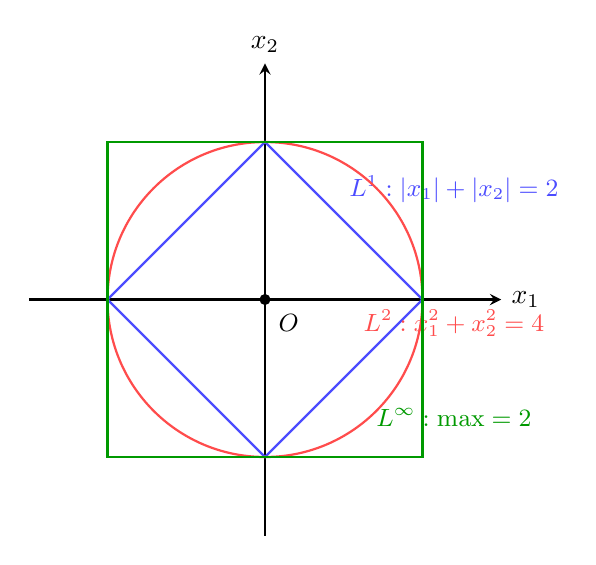
\begin{tikzpicture}[
    myaxis/.style={->, >=stealth, thick},
    mycurve/.style={thick, smooth},
    mylabel/.style={font=\small}
]
    % Axes
    \draw[myaxis] (-3, 0) -- (3, 0) node[right] {$x_1$};
    \draw[myaxis] (0, -3) -- (0, 3) node[above] {$x_2$};

    % L1 contour (diamond)
    \draw[mycurve, blue!70, thick] (0, -2) -- (2, 0) -- (0, 2) -- (-2, 0) -- cycle;
    \node[mylabel, blue!70] at (2.4, 1.4) {$L^1: |x_1|+|x_2|=2$};

    % L2 contour (circle)
    \draw[mycurve, red!70, thick] (0, 0) circle (2);
    \node[mylabel, red!70] at (2.4, -0.3) {$L^2: x_1^2+x_2^2=4$};

    % L-inf contour (square)
    \draw[mycurve, green!60!black, thick] (-2, -2) rectangle (2, 2);
    \node[mylabel, green!60!black] at (2.4, -1.5) {$L^{\infty}: \max=2$};

    % Origin
    \fill (0, 0) circle (2pt);
    \node[mylabel] at (0.3, -0.3) {$O$};
\end{tikzpicture}
\caption{二维空间中 $L^1$、$L^2$ 和 $L^{\infty}$ 范数的单位等高线。$L^1$ 范数的等高线呈菱形，易于产生稀疏解；$L^2$ 范数的等高线为圆形。}
\label{fig:vector-norms}
\end{figure}

\subsection{矩阵范数}

\begin{mydefinition}{Frobenius 范数}
矩阵 $\mathbf{A}\in\R^{m\times n}$ 的 Frobenius 范数定义为所有元素平方和的平方根：
\[
\|\mathbf{A}\|_F = \sqrt{\sum_{i=1}^{m}\sum_{j=1}^{n} A_{ij}^2}
\]
\end{mydefinition}

Frobenius 范数可以视为将矩阵展平为向量后求 $L^2$ 范数。它在深度学习中常用于衡量权重矩阵的大小，作为权重衰减（weight decay）的正则化项。

\begin{mycode}{Python中的范数计算}
\begin{lstlisting}[language=Python]
import numpy as np

x = np.array([3.0, 4.0])
A = np.array([[1, 2], [3, 4]])

# 向量范数
print(f"L1 范数: {np.linalg.norm(x, ord=1)}")
print(f"L2 范数: {np.linalg.norm(x, ord=2)}")
print(f"Linf 范数: {np.linalg.norm(x, ord=np.inf)}")

# 矩阵范数
print(f"Frobenius 范数: {np.linalg.norm(A, ord='fro')}")
print(f"Frobenius (手动): {np.sqrt(np.sum(A**2))}")
\end{lstlisting}
\end{mycode}

\section{特殊矩阵}

\subsection{正交矩阵}

若方阵 $\mathbf{Q}\in\R^{n\times n}$ 满足 $\mathbf{Q}^{\top}\mathbf{Q}=\mathbf{I}$（即 $\mathbf{Q}^{-1}=\mathbf{Q}^{\top}$），则称其为正交矩阵。正交矩阵的列向量构成一组标准正交基。

正交矩阵的一个重要性质是保范性：
\[
\|\mathbf{Q}\mathbf{x}\|_2 = \|\mathbf{x}\|_2
\]

这意味着用一个正交矩阵乘以向量不会改变向量的长度，只是旋转或反射。

\subsection{正定矩阵}

若对称矩阵 $\mathbf{A}\in\R^{n\times n}$ 满足对所有非零 $\mathbf{x}\in\R^n$ 都有 $\mathbf{x}^{\top}\mathbf{A}\mathbf{x}>0$，则称 $\mathbf{A}$ 为正定矩阵。若 $\mathbf{x}^{\top}\mathbf{A}\mathbf{x}\geq 0$，则称为半正定矩阵。

正定矩阵在深度学习中有重要应用：
\begin{itemize}
    \item \textbf{Hessian 矩阵}：若函数在某点的 Hessian 矩阵是正定的，则该点是局部极小点。
    \item \textbf{协方差矩阵}：数据集协方差矩阵总是半正定的。
    \item \textbf{牛顿法}：利用正定的 Hessian 近似来寻找最优方向。
\end{itemize}

\section{特征分解}

\subsection{特征值与特征向量}

\begin{myTheorem}{特征值与特征向量}
设 $\mathbf{A}\in\R^{n\times n}$ 为方阵。若非零向量 $\mathbf{v}\in\R^n$ 满足：
\[
\mathbf{A}\mathbf{v} = \lambda \mathbf{v}
\]
则称 $\lambda$ 为矩阵 $\mathbf{A}$ 的特征值，$\mathbf{v}$ 为对应的特征向量。
\end{myTheorem}

特征方程 $\det(\mathbf{A}-\lambda\mathbf{I})=0$ 给出了 $n$ 次特征多项式，其 $n$ 个根（可能重复或为复数）即为特征值。

\begin{example}
求矩阵 $\mathbf{A}=\begin{bmatrix} 2 & 1 \\ 1 & 2 \end{bmatrix}$ 的特征值和特征向量。

\textbf{解：}
特征方程：$\det(\mathbf{A}-\lambda\mathbf{I})=\begin{vmatrix}2-\lambda & 1 \\ 1 & 2-\lambda\end{vmatrix}=(2-\lambda)^2-1=0$

解得 $\lambda^2-4\lambda+3=0$，即 $(\lambda-1)(\lambda-3)=0$，故 $\lambda_1=1$，$\lambda_2=3$。

当 $\lambda_1=1$ 时：$(2-1)v_1+v_2=0 \Rightarrow v_1=-v_2$，取 $\mathbf{v}_1=\begin{bmatrix}1 \\ -1\end{bmatrix}$。

当 $\lambda_2=3$ 时：$(2-3)v_1+v_2=0 \Rightarrow v_2=v_1$，取 $\mathbf{v}_2=\begin{bmatrix}1 \\ 1\end{bmatrix}$。
\end{example}

\subsection{特征分解}

若方阵 $\mathbf{A}\in\R^{n\times n}$ 有 $n$ 个线性无关的特征向量 $\{\mathbf{v}_1,\ldots,\mathbf{v}_n\}$，对应特征值 $\{\lambda_1,\ldots,\lambda_n\}$，则 $\mathbf{A}$ 可以被分解为：

\[
\mathbf{A} = \mathbf{V}\boldsymbol{\Lambda}\mathbf{V}^{-1}
\]

其中 $\mathbf{V}=[\mathbf{v}_1,\mathbf{v}_2,\ldots,\mathbf{v}_n]$，$\boldsymbol{\Lambda}=\operatorname{diag}(\lambda_1,\ldots,\lambda_n)$。

特别地，若 $\mathbf{A}$ 为实对称矩阵，则存在正交矩阵 $\mathbf{Q}$ 使得：
\[
\mathbf{A} = \mathbf{Q}\boldsymbol{\Lambda}\mathbf{Q}^{\top}
\]

因为这组特征向量可以构成标准正交基，这是谱定理的特殊形式。

\begin{figure}[H]
\centering
\begin{tikzpicture}[
    mymat/.style={rectangle, draw=blue!60, fill=blue!5, minimum width=1.4cm, minimum height=1.4cm},
    mylabel/.style={font=\footnotesize},
    myeq/.style={font=\large}
]
    \node[mymat] (A) at (0, 0) {$\mathbf{A}$};
    \node[mylabel] at (0, -1) {$n\times n$};

    \node[myeq] at (1.8, 0) {$=$};

    \node[mymat] (Q) at (3.5, 0) {$\mathbf{Q}$};
    \node[mylabel] at (3.5, -1) {正交};

    \node[myeq] at (5.3, 0) {$\cdot$};

    \node[mymat] (L) at (6.8, 0) {$\boldsymbol{\Lambda}$};
    \node[mylabel] at (6.8, -1) {对角};

    \node[myeq] at (8.3, 0) {$\cdot$};

    \node[mymat] (QT) at (9.8, 0) {$\mathbf{Q}^{\top}$};
    \node[mylabel] at (9.8, -1) {正交};

    % Brackets
    \draw[decorate, decoration={brace, amplitude=8pt}, blue!60, thick]
        (Q.north west) ++(-0.2, 0.3) -- node[above=10pt, mylabel] {特征向量} (Q.north east) ++(0.2, 0.3);

    \draw[decorate, decoration={brace, amplitude=8pt}, red!60, thick]
        (L.north west) ++(-0.2, 0.3) -- node[above=10pt, mylabel] {特征值} (L.north east) ++(0.2, 0.3);

    % Geometric interpretation
    \draw[->, >=stealth, thick, blue!60] (-1, -2.5) -- (2, -2.5) node[right] {\small $\mathbf{v}_1$方向};
    \draw[->, >=stealth, thick, red!60] (-1, -2.5) -- (-1, -1.5) node[above] {\small $\mathbf{v}_2$方向};

    \node[mylabel] at (0.5, -3) {$\mathbf{A}\mathbf{v}_1=\lambda_1\mathbf{v}_1$（拉伸）};
\end{tikzpicture}
\caption{实对称矩阵的特征分解。$\mathbf{A}=\mathbf{Q}\boldsymbol{\Lambda}\mathbf{Q}^{\top}$ 表示将 $\mathbf{A}$ 的作用分解为：旋转（$\mathbf{Q}^{\top}$）、缩放（$\boldsymbol{\Lambda}$）、旋转回去（$\mathbf{Q}$）。}
\label{fig:eigendecomposition}
\end{figure}

\begin{mycode}{Python中的特征分解}
\begin{lstlisting}[language=Python]
import numpy as np

A = np.array([[2, 1],
              [1, 2]])

# 特征值和特征向量
eigenvalues, eigenvectors = np.linalg.eig(A)

print(f"特征值:\n{eigenvalues}")
print(f"特征向量:\n{eigenvectors}")

# 验证: A v = lambda v
for i in range(2):
    v = eigenvectors[:, i]
    lam = eigenvalues[i]
    print(f"\n验证特征值 {lam}:")
    print(f"A v = {A @ v}")
    print(f"lambda * v = {lam * v}")

# 实对称矩阵的特征分解重构
Q = eigenvectors   # 对实对称矩阵，特征向量自然正交
L = np.diag(eigenvalues)
A_reconstructed = Q @ L @ Q.T
print(f"\n重构矩阵:\n{A_reconstructed}")
print(f"重构误差: {np.linalg.norm(A - A_reconstructed)}")
\end{lstlisting}
\end{mycode}

\subsection{特征值与深度学习}

特征值分析在深度学习中具有重要应用：

\begin{itemize}
    \item \textbf{主成分分析（PCA）}：数据协方差矩阵的特征向量对应数据的主方向，特征值表示该方向上的方差大小。
    \item \textbf{谱归一化}：用权重矩阵的最大奇异值（奇异值是特征值的一种推广）来归一化权重，稳定GAN训练。
    \item \textbf{梯度下降的收敛性}：损失函数的 Hessian 矩阵的特征值分布影响梯度下降的收敛速度。条件数（最大特征值与最小特征值之比）越大，收敛越慢。
    \item \textbf{权重初始化}：Xavier 和 He 初始化方法基于特征值分析，确保前向传播和反向传播时信号的方差保持稳定。
\end{itemize}

\section{奇异值分解}

奇异值分解（Singular Value Decomposition, SVD）将特征分解推广到任意矩阵（不限于方阵）。

\begin{myTheorem}{奇异值分解}
对于任意矩阵 $\mathbf{A}\in\R^{m\times n}$，存在分解：
\[
\mathbf{A} = \mathbf{U}\boldsymbol{\Sigma}\mathbf{V}^{\top}
\]
其中：
\begin{itemize}
    \item $\mathbf{U}\in\R^{m\times m}$ 是正交矩阵，列向量称为左奇异向量
    \item $\mathbf{V}\in\R^{n\times n}$ 是正交矩阵，列向量称为右奇异向量
    \item $\boldsymbol{\Sigma}\in\R^{m\times n}$ 是对角矩阵，对角线元素 $\sigma_1\geq\sigma_2\geq\cdots\geq\sigma_{\min(m,n)}\geq 0$ 称为奇异值
\end{itemize}
\end{myTheorem}

SVD 的几何解释：任何矩阵 $\mathbf{A}$ 的作用可以分解为三个步骤：
\begin{enumerate}
    \item $\mathbf{V}^{\top}$：旋转（或反射）输入空间
    \item $\boldsymbol{\Sigma}$：沿坐标轴缩放（奇异值为缩放因子）
    \item $\mathbf{U}$：旋转（或反射）输出空间
\end{enumerate}

\subsection{低秩近似}

SVD 的一个重要应用是矩阵的低秩近似。保留前 $r$ 个最大的奇异值：

\[
\mathbf{A} \approx \mathbf{U}_{:,1:r} \boldsymbol{\Sigma}_{1:r,1:r} (\mathbf{V}_{:,1:r})^{\top}
\]

这是 $\mathbf{A}$ 在 Frobenius 范数意义下秩为 $r$ 的最佳近似（Eckart-Young-Mirsky 定理）。

在深度学习中，低秩近似用于：
\begin{itemize}
    \item \textbf{模型压缩}：对权重矩阵进行低秩分解减少参数。
    \item \textbf{LoRA（Low-Rank Adaptation）}：在微调大语言模型时，用低秩矩阵来近似权重更新。
    \item \textbf{推荐系统}：矩阵分解技术是协同过滤的核心。
\end{itemize}

\begin{figure}[H]
\centering
\begin{tikzpicture}[
    mymat/.style={rectangle, draw=blue!60, fill=blue!5, minimum width=1.2cm, minimum height=1.6cm},
    mydiag/.style={rectangle, draw=red!60, fill=red!5, minimum width=1.2cm, minimum height=1.6cm},
    mylabel/.style={font=\footnotesize},
    myeq/.style={font=\large}
]
    \node[mymat] (A) at (0, 0) {$\mathbf{A}$};
    \node[mylabel] at (0, -1) {$m\times n$};

    \node[myeq] at (1.8, 0) {$=$};

    \node[mymat] (U) at (3.5, 0) {$\mathbf{U}$};
    \node[mylabel] at (3.5, -1) {$m\times m$};

    \node[myeq] at (5.3, 0) {$\cdot$};

    \node[mydiag] (S) at (6.8, 0) {$\boldsymbol{\Sigma}$};
    \node[mylabel] at (6.8, -1) {$m\times n$};

    \node[myeq] at (8.3, 0) {$\cdot$};

    \node[mymat] (VT) at (9.8, 0) {$\mathbf{V}^{\top}$};
    \node[mylabel] at (9.8, -1) {$n\times n$};

    % Low-rank approximation
    \draw[->, >=stealth, thick, blue!70] (0, -2.5) -- (0, -3.5);
    \node[mylabel, blue!70] at (0.5, -3) {低秩近似};

    \node[mymat, scale=0.7] (Ur) at (3.5, -4) {$\mathbf{U}_r$};
    \node[mylabel] at (3.5, -5) {$m\times r$};

    \node[myeq, scale=0.7] at (5, -4) {$\cdot$};

    \node[mydiag, scale=0.7] (Sr) at (6.3, -4) {$\boldsymbol{\Sigma}_r$};
    \node[mylabel] at (6.3, -5) {$r\times r$};

    \node[myeq, scale=0.7] at (7.6, -4) {$\cdot$};

    \node[mymat, scale=0.7] (VTr) at (8.9, -4) {$\mathbf{V}_r^{\top}$};
    \node[mylabel] at (8.9, -5) {$r\times n$};
\end{tikzpicture}
\caption{完整的SVD与低秩近似。低秩近似仅保留前 $r$ 个最大奇异值，将存储复杂度从 $O(mn)$ 降低到 $O(r(m+n))$。}
\label{fig:svd}
\end{figure}

\begin{mycode}{Python中的SVD与低秩近似}
\begin{lstlisting}[language=Python]
import numpy as np

# 创建矩阵
np.random.seed(42)
A = np.random.randn(6, 4)

# SVD分解
U, S, Vt = np.linalg.svd(A, full_matrices=True)
print(f"奇异值: {S}")

# 重构验证
Sigma = np.zeros((6, 4))
np.fill_diagonal(Sigma, S)
A_reconstructed = U @ Sigma @ Vt
print(f"重构误差: {np.linalg.norm(A - A_reconstructed):.2e}")

# 低秩近似（保留前r个奇异值）
r = 2
U_r = U[:, :r]
S_r = np.diag(S[:r])
Vt_r = Vt[:r, :]
A_approx = U_r @ S_r @ Vt_r

print(f"\n原始矩阵:\n{A}")
print(f"\n秩-{r} 近似:\n{A_approx}")
print(f"近似误差: {np.linalg.norm(A - A_approx):.4f}")

# 信息保留比例
energy_total = np.sum(S ** 2)
energy_approx = np.sum(S[:r] ** 2)
print(f"能量保留比例: {energy_approx / energy_total:.2%}")
\end{lstlisting}
\end{mycode}

\section{Moore-Penrose 伪逆}

对于非方阵或奇异矩阵，常规的逆矩阵不存在。Moore-Penrose 伪逆（简称伪逆）提供了广义的逆矩阵概念。

\begin{mydefinition}{Moore-Penrose 伪逆}
对于矩阵 $\mathbf{A}\in\R^{m\times n}$，其伪逆 $\mathbf{A}^{+}\in\R^{n\times m}$ 定义为满足以下四个条件的唯一矩阵：
\begin{enumerate}
    \item $\mathbf{A}\mathbf{A}^{+}\mathbf{A}=\mathbf{A}$
    \item $\mathbf{A}^{+}\mathbf{A}\mathbf{A}^{+}=\mathbf{A}^{+}$
    \item $(\mathbf{A}\mathbf{A}^{+})^{\top}=\mathbf{A}\mathbf{A}^{+}$
    \item $(\mathbf{A}^{+}\mathbf{A})^{\top}=\mathbf{A}^{+}\mathbf{A}$
\end{enumerate}
\end{mydefinition}

利用 SVD，伪逆可以通过以下公式计算：

\[
\mathbf{A}^{+} = \mathbf{V}\boldsymbol{\Sigma}^{+}\mathbf{U}^{\top}
\]

其中 $\boldsymbol{\Sigma}^{+}$ 是 $\boldsymbol{\Sigma}$ 的伪逆：将非零奇异值取倒数后转置。

在实际应用中，当 $\mathbf{A}$ 可逆时，$\mathbf{A}^{+}=\mathbf{A}^{-1}$。当 $\mathbf{A}$ 列满秩时，$\mathbf{A}^{+}=(\mathbf{A}^{\top}\mathbf{A})^{-1}\mathbf{A}^{\top}$。伪逆在求解线性回归的正规方程中起到关键作用。

\section{行列式}

行列式（Determinant）将方阵映射为一个标量，记为 $\det(\mathbf{A})$ 或 $|\mathbf{A}|$。

行列式的几何意义：$\det(\mathbf{A})$ 的绝对值表示矩阵 $\mathbf{A}$ 所代表的线性变换对空间体积的缩放因子。若 $\det(\mathbf{A})=0$，则变换将空间压缩到更低维度（矩阵不可逆）。

行列式的重要性质：
\begin{itemize}
    \item $\det(\mathbf{A}\mathbf{B})=\det(\mathbf{A})\det(\mathbf{B})$
    \item $\det(\mathbf{A}^{\top})=\det(\mathbf{A})$
    \item $\det(\mathbf{A}^{-1})=1/\det(\mathbf{A})$
    \item 特征值之积：$\det(\mathbf{A})=\prod_{i}\lambda_i$
\end{itemize}

\section{迹}

矩阵的迹（Trace）是主对角线元素之和：

\[
\operatorname{tr}(\mathbf{A}) = \sum_{i=1}^{n} A_{ii}
\]

迹的重要性质：
\begin{itemize}
    \item $\operatorname{tr}(\mathbf{A}+\mathbf{B})=\operatorname{tr}(\mathbf{A})+\operatorname{tr}(\mathbf{B})$
    \item $\operatorname{tr}(c\mathbf{A})=c\operatorname{tr}(\mathbf{A})$
    \item $\operatorname{tr}(\mathbf{A}\mathbf{B})=\operatorname{tr}(\mathbf{B}\mathbf{A})$（循环置换不变性）
    \item $\operatorname{tr}(\mathbf{A})=\sum_i \lambda_i$（特征值之和）
\end{itemize}

迹在深度学习中的一个重要用途是：标量的导数可以通过迹运算技巧来简化。例如，$\nabla_{\mathbf{A}}\operatorname{tr}(\mathbf{A}\mathbf{B})=\mathbf{B}^{\top}$。

\section{PCA与SVD}

主成分分析（PCA）是降维的经典方法，其数学基础与SVD紧密相连。给定数据中心化后的矩阵 $\mathbf{X}\in\R^{m\times n}$（$m$ 个样本，$n$ 个特征），PCA的目标是找到投影方向使得投影后的方差最大。

PCA的求解步骤：
\begin{enumerate}
    \item 对数据去中心化（减去均值）
    \item 计算协方差矩阵 $\mathbf{C}=\frac{1}{m-1}\mathbf{X}^{\top}\mathbf{X}$
    \item 对 $\mathbf{C}$ 进行特征分解，取前 $k$ 个最大特征值对应的特征向量作为主成分
\end{enumerate}

等价地，可以直接对 $\mathbf{X}$ 进行SVD：$\mathbf{X}=\mathbf{U}\boldsymbol{\Sigma}\mathbf{V}^{\top}$，则 $\mathbf{V}$ 的前 $k$ 列即为前 $k$ 个主成分方向。

\begin{mycode}{Python中的PCA实现}
\begin{lstlisting}[language=Python]
import numpy as np
import matplotlib.pyplot as plt

np.random.seed(42)
# 生成二维数据（有相关性的数据）
n_samples = 200
mean = [3, 4]
cov = [[2.0, 1.5],
       [1.5, 1.0]]
X = np.random.multivariate_normal(mean, cov, n_samples)

# 1. 去中心化
X_centered = X - X.mean(axis=0)

# 2. 协方差矩阵
C = (X_centered.T @ X_centered) / (n_samples - 1)

# 3. 特征分解
eigenvalues, eigenvectors = np.linalg.eig(C)

# 按特征值降序排列
idx = eigenvalues.argsort()[::-1]
eigenvalues = eigenvalues[idx]
eigenvectors = eigenvectors[:, idx]

print(f"特征值: {eigenvalues}")
print(f"主成分方向:\n{eigenvectors}")

# 4. 投影到第一主成分
X_pca = X_centered @ eigenvectors[:, :1]
print(f"降维后数据形状: {X_pca.shape}")

# 5. 使用SVD方法（等价）
U, S, Vt = np.linalg.svd(X_centered, full_matrices=False)
principal_components_svd = Vt[:1, :].T  # 第一主成分
print(f"SVD方法的主成分方向:\n{principal_components_svd}")

# 解释方差比例
explained_variance_ratio = eigenvalues / eigenvalues.sum()
print(f"各主成分解释方差比例: {explained_variance_ratio}")
\end{lstlisting}
\end{mycode}

\begin{figure}[H]
\centering
\begin{tikzpicture}[
    mypoint/.style={circle, fill=blue!40, inner sep=1pt},
    myarrow/.style={->, >=stealth, very thick},
    mylabel/.style={font=\small}
]
    % Coordinate axes
    \draw[->, >=stealth, gray, thin] (-2, -2) -- (6, -2);
    \draw[->, >=stealth, gray, thin] (-2, -2) -- (-2, 6);

    % Data cluster (ellipse)
    \draw[blue!30, fill=blue!5, rotate around={30:(2,2)}] (2, 2) ellipse (3cm and 1.2cm);

    % Center
    \fill[red] (2, 2) circle (3pt);
    \node[mylabel, red] at (2.3, 2.3) {均值};

    % PC1
    \draw[myarrow, red!80, rotate around={30:(2,2)}]
        (2, 2) -- (2, 5) node[above] {\small PC1};

    % PC2
    \draw[myarrow, blue!80, rotate around={30:(2,2)}]
        (2, 2) -- (5, 2) node[right] {\small PC2};

    % Data points
    \foreach \i in {0, 10, ..., 350} {
        \pgfmathsetmacro{\x}{2 + 2.5*cos(\i)*cos(30) - 0.8*sin(\i)*sin(30)}
        \pgfmathsetmacro{\y}{2 + 2.5*cos(\i)*sin(30) + 0.8*sin(\i)*cos(30)}
        \node[mypoint] at (\x, \y) {};
    }

    \node[mylabel] at (4, -1) {PC1方向 = 最大方差方向};
    \node[mylabel, blue!80] at (5.5, 1) {PC2方向（与PC1正交）};
\end{tikzpicture}
\caption{PCA主成分方向的几何解释。PC1是数据方差最大的方向，PC2与PC1正交且方差次之。}
\label{fig:pca}
\end{figure}

\section{向量与矩阵微积分}

在后续章节中，我们将频繁使用矩阵微积分。这里给出常用公式。

对于向量和矩阵的导数，有：

\begin{itemize}
    \item $\nabla_{\mathbf{x}}(\mathbf{a}^{\top}\mathbf{x}) = \mathbf{a}$
    \item $\nabla_{\mathbf{x}}(\mathbf{x}^{\top}\mathbf{A}\mathbf{x}) = (\mathbf{A}+\mathbf{A}^{\top})\mathbf{x}$
    \item $\nabla_{\mathbf{x}}\|\mathbf{x}\|_2^2 = 2\mathbf{x}$
    \item $\nabla_{\mathbf{A}}(\operatorname{tr}(\mathbf{A}\mathbf{B})) = \mathbf{B}^{\top}$
    \item $\nabla_{\mathbf{A}}(\det(\mathbf{A})) = \det(\mathbf{A})(\mathbf{A}^{-1})^{\top}$
\end{itemize}

这些公式将在推导梯度下降、正规方程和反向传播时反复出现。

\section{本章小结}

本章介绍了深度学习所需的线性代数基础知识。核心概念包括：
\begin{itemize}
    \item 标量、向量、矩阵和张量是多维数组的分层抽象
    \item 矩阵乘法是神经网络前向传播的基本运算
    \item 范数用于衡量向量和矩阵的大小，在正则化中起关键作用
    \item 特征分解揭示了矩阵的本质结构，SVD将其推广到任意矩阵
    \item PCA利用特征分解实现数据降维
    \item SVD的低秩近似在模型压缩中具有重要应用
\end{itemize}

牢固掌握这些线性代数知识，将为理解深度学习的数学本质打下坚实的基础。
